\documentclass[a4paper, 12pt, twoside]{article}
\usepackage{estilo}

% ── Margens laterais estritamente oficiais (2.5cm) conforme edital EU ──
\geometry{
  a4paper,
  inner=2.5cm, outer=2.5cm,
  top=1.9cm, bottom=1.4cm,
  headheight=40pt, headsep=10pt
}
\setstretch{0.80}
\setlength{\parindent}{0.65cm}
\setlength{\textfloatsep}{2pt plus 1pt minus 1pt}
\setlength{\intextsep}{2pt plus 1pt minus 1pt}
\setlength{\abovecaptionskip}{1.5pt}
\setlength{\belowcaptionskip}{1.5pt}
% Compactar espaços de equações
\setlength{\abovedisplayskip}{3pt plus 1pt minus 1pt}
\setlength{\belowdisplayskip}{3pt plus 1pt minus 1pt}
\setlength{\abovedisplayshortskip}{1pt plus 0pt minus 1pt}
\setlength{\belowdisplayshortskip}{2pt plus 1pt minus 1pt}

\renewcommand{\topfraction}{0.95}
\renewcommand{\bottomfraction}{0.95}
\renewcommand{\textfraction}{0.05}
\renewcommand{\floatpagefraction}{0.90}

\title{O Papel da Causalidade Temporal e da Rigidez Numérica na Falha de PINNs para Padrões de Turing: Uma Análise Crítica do Modelo de Schnakenberg}

\author{%
  Autor Principal\authorinfo{autor@alu.ufc.br} \\
  Orientador\authorinfo{orientador@ufc.br}
}
\date{}

\begin{document}
\maketitle

%%%%%%%%%%%%%%%%%%%%% RESUMO E ABSTRACT %%%%%%%%%%%%%%%%%%%%%%%%%%%%%%

\qabstract{Resumo}{Palavras-chave}{ODS}{%
Este trabalho investiga as causas fundamentais pelas quais as Redes Neurais Informadas por Física (PINNs) em formulação padrão contínua falham na simulação direta (\textit{forward}) de padrões de Turing no modelo de reação-difusão de Schnakenberg. Com base nos parâmetros exatos da tese de \textcite{pereira2019} ($D_v/D_u = 20$, $\kappa = 100$ no domínio unitário $\Omega = [0, 1]^2$), conduziram-se experimentos com um Perceptron Multicamadas (MLP) de $5$ camadas ocultas ($66.818$ parâmetros) treinado por $20.000$ épocas via otimizador Adam na GPU. Demonstra-se o paradoxo da convergência espúria: a despeito de atingir perda residual global reduzida ($\mathcal{L}_{\mathrm{total}} = 1{,}95 \times 10^{-4}$) e resíduo inicial quase nulo ($\mathcal{L}_{\mathrm{ic}} = 4{,}02 \times 10^{-8}$), a rede colapsa integralmente para o estado estacionário homogêneo trivial ($u^* = 0{,}90$), incorrendo em um erro relativo $L_2$ de $60{,}85\%$ em relação à referência. Identificam-se três patologias estruturais: (i) a quebra da causalidade temporal pela amostragem global em $\Omega \times [0, T]$, onde a retropropagação (\textit{backpropagation}) de resíduos futuros suprime perturbações pretéritas; (ii) a rigidez cinética reativa; e (iii) o viés espectral da MLP contra modos de alta frequência. Em contrapartida, revisita-se o Método de Diferenças Finitas (MDF) com Direções Alternadas Implícitas (ADI) linearizado de \textcite{pereira2019}, cuja marcha temporal causal estrita assegura estabilidade incondicional $\mathcal{O}(\Delta t^2)$ e resolução exata das manchas periódicas (\textit{spots}) em $9{,}59$\,s.%
}{%
redes neurais informadas por física; causalidade temporal; instabilidade de turing; modelo de schnakenberg; rigidez numérica; método de diferenças finitas; direções alternadas implícitas%
}{%
indústria, inovação e infraestrutura%
}

\qabstract{Abstract}{Keywords}{SDG}{%
This work investigates the fundamental causes behind the failure of standard continuous Physics-Informed Neural Networks (PINNs) in forward simulations of Turing patterns in the Schnakenberg reaction-diffusion model. Based on the exact benchmark parameters from the thesis of \textcite{pereira2019} ($D_v/D_u = 20$, $\kappa = 100$ on the unit domain $\Omega = [0, 1]^2$), experiments were carried out using a deep Multi-Layer Perceptron (MLP) with $5$ hidden layers ($66,818$ trainable parameters) trained for $20,000$ epochs with Adam on GPU. We demonstrate the spurious convergence paradox: despite reaching a very low global residual loss ($\mathcal{L}_{\mathrm{total}} = 1.95 \times 10^{-4}$) and negligible initial condition residual ($\mathcal{L}_{\mathrm{ic}} = 4.02 \times 10^{-8}$), the network collapses into the trivial homogeneous steady state ($u^* = 0.90$), yielding a relative $L_2$ error of $60.85\%$ against the reference solution. Three structural pathologies are identified: (i) violation of temporal causality via global space-time collocation, where error backpropagation from future states suppresses past perturbations; (ii) kinetic stiffness; and (iii) spectral bias against critical wavenumbers. In contrast, we revisit the Finite Difference Method (FDM) with Linearized Alternating Direction Implicit (ADI) time-stepping from \textcite{pereira2019}, whose strictly causal marching guarantees unconditional $\mathcal{O}(\Delta t^2)$ stability and exact periodic spot formation in $9.59$\,s.%
}{%
physics-informed neural networks; temporal causality; turing instability; schnakenberg model; numerical stiffness; finite difference method; alternating direction implicit%
}{%
industry, innovation and infrastructure%
}

%%%%%%%%%%%%%%%%%%%%%%%%%%%%%% SEÇÕES %%%%%%%%%%%%%%%%%%%%%%%%%%%%%

\section{Introdução}

A emergência espontânea de estruturas periódicas e quebras de simetria em sistemas de reação-difusão, concebida por Alan Turing em seu trabalho seminal \parencite{turing1952morphogenesis}, fundamenta a compreensão da morfogênese biológica e dos processos de auto-organização não linear \parencite{murray2003mathbio}. No modelo canônico de Schnakenberg \parencite{schnakenberg1979simple}, cinéticas reativas trimoleculares acopladas a taxas de difusão desiguais ($D_v \gg D_u$) amplificam perturbações imperceptíveis na escala inicial ($\sim 10^{-3}$), reorganizando o meio homogêneo em redes periódicas de manchas (\textit{spots}).

Com os avanços do aprendizado científico de máquina, as Redes Neurais Informadas por Física (PINNs) \parencite{raissi2019pinns} consolidaram-se como um paradigma contínuo e livre de malha (\textit{meshless}). Ao embutir os operadores diferenciais da Equação Diferencial Parcial (EDP) no funcional de perda via diferenciação automática (\textit{autograd}), as PINNs aproximam soluções no espaço-tempo global. Todavia, a formulação padrão de PINNs enfrenta graves entraves diante de \textbf{sistemas regidos por instabilidades dinâmicas e bifurcações espaciais}.

Em simulações diretas (\textit{forward}) de padrões de Turing, constata-se um paradoxo empírico: a rede atinge resíduos globais diminutos ($\mathcal{L} < 10^{-3}$), mas o campo predito permanece estagnado no equilíbrio homogêneo trivial, suprimindo os padrões morfogênicos. Este artigo analisa os mecanismos físico-matemáticos desse colapso no modelo de Schnakenberg, adotando como base a formulação de \textcite{pereira2019}. Demonstra-se como a \textbf{quebra da causalidade temporal}, a \textbf{rigidez reativa} ($\kappa = 100$) e o \textbf{viés espectral} aprisionam a rede no estado plano. Em paralelo, comprova-se a superioridade da marcha causal sequencial do \textbf{Método de Diferenças Finitas (MDF)} com \textbf{Direções Alternadas Implícitas (ADI)} linearizado \parencite{pereira2019}.

\section{Desenvolvimento}

\subsection{Fundamentação Teórica}

\textbf{Modelo de Reação-Difusão de Schnakenberg:} No domínio unitário bidimensional $\Omega = [0, 1]^2\,\text{m}^2$ sob contornos de fluxo nulo $\nabla u \cdot \mathbf{n} = \nabla v \cdot \mathbf{n} = 0$ em $\partial\Omega$, o modelo é regido pelo par acoplado \parencite{schnakenberg1979simple, pereira2019}:
\begin{equation}
  \frac{\partial u}{\partial t} = D_u \nabla^2 u + \kappa \left( a - u + u^2 v \right), \quad
  \frac{\partial v}{\partial t} = D_v \nabla^2 v + \kappa \left( b - u^2 v \right), \label{eq:schnak}
\end{equation}
onde $u, v$ são concentrações de ativador e inibidor, $D_u, D_v$ os coeficientes difusivos, $a, b > 0$ constantes cinéticas e $\kappa$ a escala de reação. O equilíbrio homogêneo $(u^*, v^*)$ satisfaz $u^* = a + b$, $v^* = b / (a + b)^2$ \parencite{pereira2019}.

Pela Análise Linear de Estabilidade (LSA) com perturbações periódicas proporcionais a $e^{\lambda t} \cos(k_x x) \cos(k_y y)$, a matriz Jacobiana da reação em $(u^*, v^*)$ é dada por \parencite{murray2003mathbio}:
\begin{equation}
  J = \begin{pmatrix} f_u & f_v \\ g_u & g_v \end{pmatrix} = \begin{pmatrix} \frac{b - a}{a + b} & (a + b)^2 \\ -\frac{2b}{a + b} & -(a + b)^2 \end{pmatrix}.
\end{equation}
Para a emergência de instabilidade de Turing impulsionada por difusão, quatro condições devem coexistir \parencite{murray2003mathbio, pereira2019}:
\begin{equation}
  \mathrm{Tr}(J) < 0, \quad \det(J) > 0, \quad D_v f_u + D_u g_v > 0, \quad \left( D_v f_u + D_u g_v \right)^2 > 4 D_u D_v \det(J).
\end{equation}
Sob essas condições, perturbações no entorno do modo crítico $k_c^2 \approx 135\,\text{rad}^2/\text{m}^2$ sofrem amplificação exponencial $\propto e^{\lambda(k^2) t}$ com $\mathrm{Re}(\lambda) > 0$, quebrando a simetria espacial e gerando os \textit{spots}.

\textbf{O Esquema MDF ADI Semi-Implícito Linearizado:} Para superar a rigidez temporal preservando a causalidade física, \textcite{pereira2019} formulou o método ADI linearizado de Peaceman-Rachford ($n \to n+1/2 \to n+1$):
\begin{align}
  \left(I - \tfrac{D_u \Delta t}{2}\delta_x^2\right) u^{n+1/2} &= \left(I + \tfrac{D_u \Delta t}{2}\delta_y^2\right) u^n + \tfrac{\Delta t}{2} \kappa \tilde{f}^{n+1/2}, \label{eq:adi_u} \\
  \left(I - \tfrac{D_u \Delta t}{2}\delta_y^2\right) u^{n+1} &= \left(I + \tfrac{D_u \Delta t}{2}\delta_x^2\right) u^{n+1/2} + \tfrac{\Delta t}{2} \kappa \tilde{f}^{n+1/2}, \label{eq:adi_v}
\end{align}
onde $\tilde{f}^{n+1/2}$ é o termo reativo predito linearizado em $t^{n+1/2}$ por Taylor de segunda ordem \parencite{pereira2019}. Esse esquema desacopla as coordenadas em matrizes tridiagonais $\mathcal{O}(N)$ resolvidas pelo Algoritmo de Thomas, com estabilidade incondicional e ordem $\mathcal{O}(\Delta t^2)$ \parencite{pereira2019}.

\textbf{Arquitetura PINN, Autograd e Retropropagação:} A PINN parametriza $\hat{\mathbf{w}}_\theta = [\hat{u}_\theta, \hat{v}_\theta]^\top$ via MLP sobre $\mathbf{z} = [x, y, t]^\top \in \Omega \times [0, T]$ em $L = 5$ camadas ocultas com largura $d_h = 128$ ($N_\theta = 66.818$ pesos) e ativação $\sigma(z) = \tanh(z) \in C^\infty(\mathbb{R})$:
\begin{equation}
  \mathbf{h}_1 = \sigma\left(\mathbf{W}_1 \mathbf{z} + \mathbf{b}_1\right), \quad \mathbf{h}_\ell = \sigma\left(\mathbf{W}_\ell \mathbf{h}_{\ell-1} + \mathbf{b}_\ell\right) \; (\ell=2,\dots,L), \quad \hat{\mathbf{w}}_\theta(\mathbf{z}) = \mathbf{W}_{L+1} \mathbf{h}_L + \mathbf{b}_{L+1}.
\end{equation}
O treinamento combina dois fluxos: (i) a \textbf{diferenciação automática (\textit{autograd})} em relação a $\mathbf{z}$ para obter derivadas parciais da EDP ($\frac{\partial \hat{u}}{\partial t}, \nabla^2 \hat{u}, \frac{\partial \hat{v}}{\partial t}, \nabla^2 \hat{v}$) sem malha \parencite{raissi2019pinns}; e (ii) a \textbf{retropropagação (\textit{backpropagation})} de $\mathcal{L}(\theta)$ para atualizar os parâmetros $\theta$ via otimizador estocástico. O funcional multiobjetivo $L_2$ é expresso por:
\begin{align}
  \mathcal{L}(\theta) &= \frac{1}{N_f}\sum_{i=1}^{N_f} \left(\|\mathcal{R}_u^{(i)}\|^2 + \|\mathcal{R}_v^{(i)}\|^2\right) + \frac{\lambda_{\mathrm{ic}}}{N_0}\sum_{j=1}^{N_0} \|\hat{\mathbf{w}}_0^{(j)} - \mathbf{w}_0^{(j)}\|^2 \nonumber \\
  &\quad + \frac{\lambda_{\mathrm{bc}}}{N_b}\sum_{k=1}^{N_b} \left(\|\nabla\hat{u}^{(k)}\cdot\mathbf{n}\|^2 + \|\nabla\hat{v}^{(k)}\cdot\mathbf{n}\|^2\right), \label{eq:loss_pinn}
\end{align}
onde $\mathcal{R}_u = \frac{\partial \hat{u}}{\partial t} - D_u \nabla^2 \hat{u} - \kappa(a - \hat{u} + \hat{u}^2 \hat{v})$ e $\mathcal{R}_v = \frac{\partial \hat{v}}{\partial t} - D_v \nabla^2 \hat{v} - \kappa(b - \hat{u}^2 \hat{v})$.

\subsection{Metodologia}

Adotaram-se os parâmetros canônicos formalizados na tese de \textcite[Cap.~2 e 4]{pereira2019}, sintetizados na Tabela~\ref{tab:parametros}. O domínio espacial corresponde a $\Omega = [0, 1]^2$ e o horizonte temporal a $t \in [0, 2{,}0\,\text{s}]$.

\begin{table}[ht]
\caption{Parâmetros físicos, dimensionais e hiperparâmetros de rede adotados conforme \textcite{pereira2019}.}
\label{tab:parametros}
\centering
\footnotesize
\setlength{\tabcolsep}{2.5pt}
\begin{tabular}{p{2.2cm}p{8.0cm}p{4.8cm}}
\toprule
\textbf{Parâmetro} & \textbf{Descrição Física / Numérica} & \textbf{Valor Adotado} \\
\midrule
$\Omega, \; T$ & Domínio espacial e horizonte temporal & $[0, 1]^2\,\text{m}^2, \quad T = 2{,}0\,\text{s}$ \\
$a, \; b, \; \kappa$ & Parâmetros cinéticos da reação & $a = 0{,}1305, \; b = 0{,}7695, \; \kappa = 100{,}0$ \\
$D_u, \; D_v$ & Coeficientes de difusão ($D_v/D_u = 20$) & $D_u = 0{,}05, \; D_v = 1{,}00$ \\
$(u^*, \; v^*)$ & Equilíbrio estacionário homogêneo & $(0{,}9000, \; 0{,}9500)$ \\
$N_f, \; N_0, \; N_b$ & Pontos de colocação (EDP, IC e BC Neumann) & $10.000, \quad 2.500, \quad 2.000$ \\
Arquitetura MLP & Camadas ocultas e neurônios & $5 \times 128 \text{ neurônios } (66.818 \text{ pesos})$ \\
Otimizador & Adam com Cosine Annealing & $20.000$ épocas ($19{,}5$\,min GPU) \\
\bottomrule
\end{tabular}
\caption*{Fonte: Elaboração própria com base em \textcite{pereira2019}.}
\end{table}

A condição inicial é uma perturbação gaussiana de amplitude $\epsilon = 10^{-3}$ centrada em $(1/3, 1/2)$ \parencite{pereira2019}:
\begin{equation}
  u(x, y, 0) = u^* + 10^{-3} e^{-100\left[(x - 1/3)^2 + (y - 1/2)^2\right]}, \quad v(x, y, 0) = v^*. \label{eq:ic_gauss}
\end{equation}
O treinamento foi executado por $20.000$ épocas em GPU (NVIDIA RTX 3050, tempo total de $19{,}49$\,min). A solução numérica de referência foi gerada pelo resolvedor MDF ADI linearizado de \textcite{pereira2019} em malha de $128 \times 128$ nós com $\Delta t = 10^{-3}\,\text{s}$.

\subsection{Resultados e Discussão}

\textbf{O Paradoxo da Convergência Espúria e Heterogeneidade Temporal:} A Figura~\ref{fig:loss_hetero}(a) ilustra a convergência das perdas ao longo das 20.000 épocas. A perda total atinge $\mathcal{L}_{\mathrm{total}} = 1{,}95 \times 10^{-4}$, com $\mathcal{L}_{\mathrm{ic}} = 4{,}02 \times 10^{-8}$. Contudo, a amplitude de heterogeneidade $\|u(t) - u^*\|_{L_2}$ (Figura~\ref{fig:loss_hetero}(b)) comprova o colapso: enquanto o MDF ADI exibe amplificação exponencial e saturação nos \textit{spots}, a PINN converge para a solução plana $u(x,y,t) \equiv u^* = 0{,}9000$.

\begin{figure}[!ht]
\caption{Dinâmica de treinamento e heterogeneidade: (a) convergência das componentes de perda $\mathcal{L}(\theta)$ da PINN ao longo de 20.000 épocas; e (b) evolução temporal da amplitude $\|u(t) - u^*\|_{L_2}$ evidenciando o crescimento físico no MDF ADI \parencite{pereira2019} versus o colapso no atrator trivial na PINN.}
\label{fig:loss_hetero}
\centering
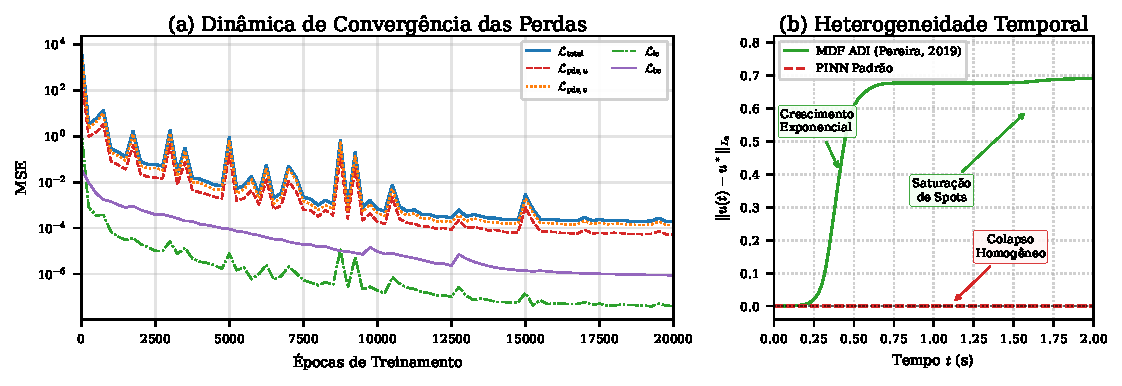
\includegraphics[width=1.0\textwidth]{figures/fig_loss_heterogeneity_duo.pdf}\\
{\footnotesize Fonte: Elaboração própria.}
\end{figure}

\textbf{Mecanismos Físico-Matemáticos da Falha da PINN:} Três patologias explicam esse aprisionamento:

\textit{1. Quebra da Causalidade Temporal e Retropropagação Espúria:} Na física real, a evolução temporal é estritamente causal. No treinamento da PINN, a amostragem ocorre simultaneamente em $\Omega \times [0, T]$. Como $(u^*, v^*)$ zera a reação e a difusão, ele anula os resíduos da EDP para $t \gg 0$. Durante a retropropagação (\textit{backpropagation}), esses gradientes associados a instantes futuros propagam-se através dos parâmetros $\theta$ até $t=0$, funcionando como uma viscosidade numérica espúria que dissipa a perturbação inicial $\epsilon \sim 10^{-3}$ antes da amplificação física.

\textit{2. Rigidez Cinética e Domínio no Hessiano:} Com $\kappa = 100$, a escala reativa $\tau_{\mathrm{reac}} \sim 0{,}01\,\text{s}$ é muito mais veloz que a difusiva $\tau_{\mathrm{dif}} \sim 20\,\text{s}$. O gradiente $\nabla_\theta \mathcal{L}_{\mathrm{pde}}$ é dominado pela reação, impondo o equilíbrio antes que a difusão segregue espécies.

\textit{3. Viés Espectral contra Modos Críticos:} MLPs exibem viés espectral que prioriza baixas frequências espaciais. Como o modo de Turing reside em alta frequência ($k_c^2 \approx 135\,\text{rad}^2/\text{m}^2$), a rede amortece as oscilações dos padrões.

\textbf{Confronto com o MDF ADI Linearizado de Pereira (2019):} A Figura~\ref{fig:snapshots_profile} e a Tabela~\ref{tab:comparativo} detalham o confronto direto. O MDF ADI de \textcite{pereira2019} captura a expansão em $t=0{,}02$\,s, a quebra de simetria em $t=0{,}41$\,s e a cristalização dos \textit{spots} em $t=2{,}00$\,s ($u \in [0{,}2134;\, 2{,}8305]$) em $9{,}59$\,s. A PINN consome $19{,}49$\,min em GPU e permanece estagnada em $u \approx 0{,}9000$, com erro relativo $L_2$ de $60{,}85\%$.

\begin{table}[ht]
\caption{Síntese comparativa metodológica e quantitativa: PINN Padrão versus MDF ADI Linearizado \parencite{pereira2019}.}
\label{tab:comparativo}
\centering
\footnotesize
\setlength{\tabcolsep}{2.5pt}
\begin{tabular}{p{3.4cm}p{5.7cm}p{5.7cm}}
\toprule
\textbf{Critério de Avaliação} & \textbf{PINN Padrão (20.000 Épocas)} & \textbf{MDF ADI Linearizado \parencite{pereira2019}} \\
\midrule
Integração Temporal & Espaço-tempo contínuo $\Omega \times [0, T]$ & Marcha sequencial causal ($t^n \to t^{n+1}$) \\
Causalidade Física & Violada (retropropagação de resíduos futuros) & Estritamente preservada \\
Sensibilidade à Perturbação & Dissipada (atração para o estado plano) & Amplificada $\propto e^{\lambda t}$ (instabilidade real) \\
Resolução Numérica & Autograd e retropropagação ($66.818$ pesos) & Algoritmo de Thomas $\mathcal{O}(N)$ tridiagonal \\
Perda Residual / Erro & $\mathcal{L}_{\mathrm{total}} = 1{,}95 \times 10^{-4}$ (Erro $L_2 = 60{,}85\%$) & Precisão $\mathcal{O}(\Delta t^2)$, convergente \\
Tempo Computacional & GPU ($1.169{,}48$\,s / $19{,}49$\,min) & CPU ($9{,}59$\,s em $128 \times 128$) \\
Faixa $u(t=2{,}00\,\text{s})$ & $u \in [0{,}8994;\, 0{,}9001]$ (Colapso uniforme) & $u \in [0{,}2134;\, 2{,}8305]$ (\textit{Spots} nítidos) \\
\bottomrule
\end{tabular}
\caption*{Fonte: Elaboração própria.}
\end{table}

\begin{figure}[!ht]
\caption{Confronto espaço-temporal e perfil transversal: (a) concentração 2D do ativador $u(x,y,t)$ via MDF ADI \parencite{pereira2019} (linha superior) versus PINN Padrão (linha inferior) em $t \in \{0{,}02;\, 0{,}41;\, 2{,}00\}\,\mathrm{s}$; e (b) corte transversal horizontal em $y=0{,}5\,\mathrm{m}$ no instante final $t=2{,}0\,\mathrm{s}$.}
\label{fig:snapshots_profile}
\centering
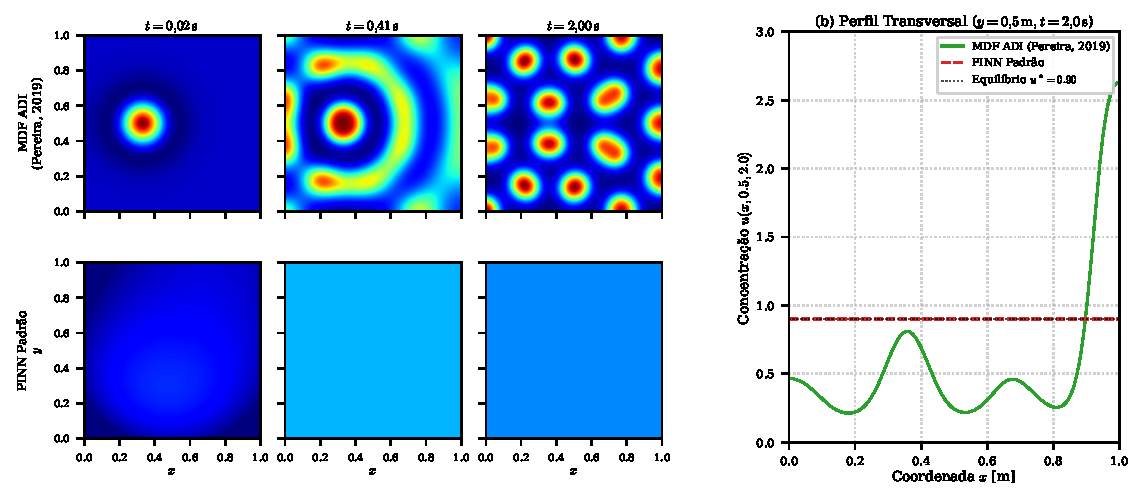
\includegraphics[width=1.0\textwidth]{figures/fig_combined_snapshots_profile.pdf}\\
{\footnotesize Fonte: Elaboração própria.}
\end{figure}

\section{Considerações Finais}

A investigação demonstra que o colapso de PINNs padrão na simulação de padrões de Turing decorre de patologias intrínsecas causadas pela violação da causalidade temporal, rigidez cinética e viés espectral. A amostragem global em $\Omega \times [0, T]$ converte o estado estacionário plano em um atrator espúrio de perda residual diminuta ($\sim 10^{-4}$), dissipando a instabilidade física via retropropagação de gradientes futuros. Em contrapartida, o método MDF ADI linearizado de \textcite{pereira2019} comprova que a marcha causal sequencial é indispensável para sistemas morfogênicos, resolvendo a bifurcação em $9{,}59$\,s. Conclui-se que, para tornar PINNs viáveis em problemas de Turing, é imperativo adotar pesagens causais temporais, marcha discreta no tempo ou esquemas de continuação em $\kappa$.

\renewcommand*{\bibfont}{\footnotesize}
\setlength{\bibitemsep}{0pt}
\setlength{\bibparsep}{-1pt}
\begin{refcontext}[sorting=none]
\printbibliography
\end{refcontext}

\end{document}
